\documentclass[10pt]{exam}
\usepackage[icp]{template-for-exam}
\usepackage{pgfplots}
\pgfplotsset{compat=1.18}

\title{Drawing a Wave}
\author{Rohrbach}
\date{\today}

\begin{document}
\maketitle

\begin{questions}
  \question
    Draw each of these three transverse waves:

    \newcommand{\makegraph}{
      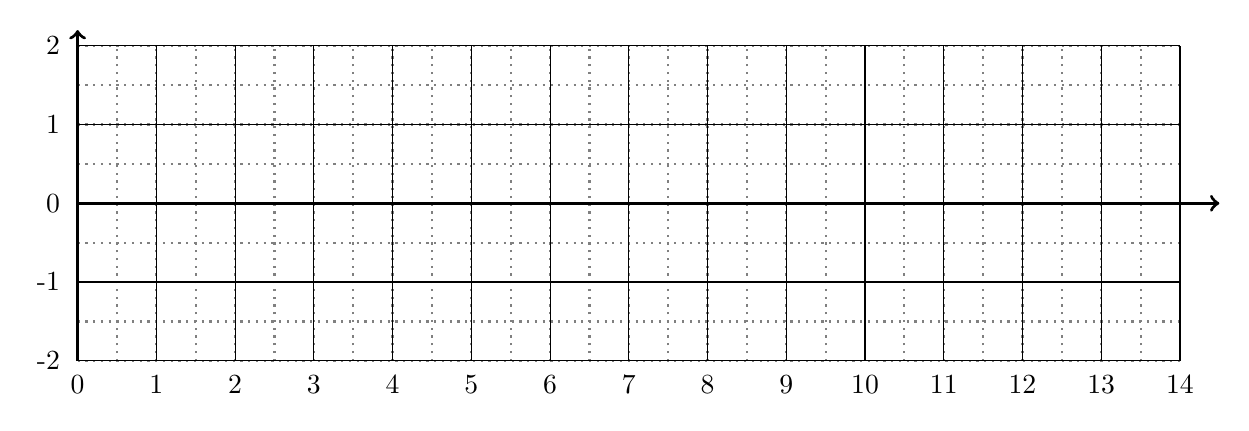
\begin{tikzpicture}
        \def\ymax{2}
        \def\xmax{14}
        \draw[dotted,thick,gray] 
          (0,-\ymax*1cm) grid[step=0.5cm] (\xmax*1cm,\ymax*1cm);
        \draw 
          (0,-\ymax*1cm) grid[step=1cm] (\xmax*1cm,\ymax*1cm);
        \foreach \x in {0,...,\xmax}{
          \draw (\x*1cm,-\ymax*1cm) ++(0,-.3cm) node {\x};
        }
        \foreach \y in {-\ymax,...,\ymax}{
          \node[anchor=east] at (-0.1cm,\y*1cm) {\y};
        }
        \draw[very thick,->] 
          (0,0) -- (\xmax*1cm,0) -- ++(0.5cm,0);
        \draw[very thick,->] 
          (0,-\ymax*1cm) -- (0,\ymax*1cm) -- ++(0,0.2cm);
      \end{tikzpicture}
    }

    \paragraph{Wave \#1} 
      Amplitude = 1 cm; Wavelength = 2 cm

    \makegraph

    \paragraph{Wave \#2}
      Amplitude = 2 cm; Wavelength = 4 cm

    \makegraph

    \paragraph{Wave \#3}
      Amplitude = 1.5 cm; Wavelength = 3 cm

    \makegraph

  \question
    On each wave, label {\bf one} of each of the following:

    \begin{checkboxes}
      \choice crest
      \choice trough
      \choice amplitude
      \choice wavelength
    \end{checkboxes}

  \pagebreak

  \question
    How can you tell that each of the waves you drew are transverse?
    \vs

  \question
    If all of these waves were traveling at the same speed, which one would have the {\bf highest frequency}?  How do you know? \label{freq}
    \vs

  \question
    Assume that each wave is traveling at 27 cm/s.  Calculate the frequency of each wave.  (Recall the equation $v=f\lambda$) \label{calc}

    \renewcommand{\ku}[1][7em]{
      \begin{tabular}
        {p{.2\textwidth}|p{.35\textwidth}|p{.15\textwidth}}
        \small Knowns/Unknowns    &
        \small  Plug \& Chug      & 
        \small Answer w/ Units \\
        &&\\[#1]
      \end{tabular}
}

    \begin{parts}
      \part Wave \#1 

      \ku
      
      \part Wave \#2 
      
      \ku

      \part Wave \#3 
      
      \ku

    \end{parts}

  \question
    Do your calculations in question \ref{calc} agree with your answer in question \ref{freq}?  Explain.
    \vs


\end{questions}

\end{document}